\section{Results}

\figureref{fig.experiment.mortality} gives an overview how many respondents we
had to our pretest, posttest, and follow-up questions. As seen in the figure
the non-achievement rate was quite high from the initial population $n_1$ to
the respondents of our pretest $n_2$. The non-achievement
rates was more or less constant from pretest respondents $n_2$ to treatment
$t_1$ and placebo $p_1$ obtention, to successful treatment $t_2$ and placebo
$p_2$ installation, and finally to posttest respondents $t_3$ and $p_3$.
The non-achievement rate for going trough
all steps from a pretest ($N = 123$) to the posttest ($N = 14 + 11 = 25$)
\begin{sparkline}{3}
  %Name  Size Unit
  %pre   100%  1
  %post 20.3%  .203
  \sparkspike .25  1
  \sparkspike .75  .203
\end{sparkline}
is quite high at 79.7\%.

\newcommand{\threeguides}{%
  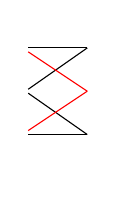
\begin{tikzpicture}
    \draw (-1,1) -- (-1,1);
      \draw (-1,0.75) -- (-0.25,0.75);
      \draw (-1,0.225) -- (-0.25,0.75);
      \draw (-1,0.175) -- (-0.25,-0.35);
      \draw (-1,-0.35) -- (-0.25,-0.35);
    \begin{scope}[color=red]
      \draw (-1,0.70) -- (-0.25,0.2);
      \draw (-1,-0.30) -- (-0.25,0.2);
    \end{scope}
    \draw (-1,-1) -- (-1,-1);
  \end{tikzpicture}}

\begin{table}
  \begin{whole}
  \begin{tabular}{rrrrrrrrrrl}

    &
    &
    \multicolumn{2}{c}{Gender (\%)} \\

    &
    \multicolumn{1}{c}{$N$} &
    \multicolumn{1}{c}{female} &
    \multicolumn{1}{c}{male} &
    \multicolumn{1}{c}{$\overline{Age}$} &
    \multicolumn{1}{c}{$\sigma$} &
    &
    \multicolumn{1}{c}{$U$} &
    \multicolumn{1}{c}{$Z$} &
    \multicolumn{1}{c}{$p$ (2-tailed)} \\

    \cmidrule(lr){2-10}

    $E$ &
    13 &
    14.3 &
    85.7 &
    26.23 &
    10.902 &
    \multirow{3}{*}{\threeguides} &
    68.5 &
    -0.174 &
    0.876 &
    $E$\dash{}$C$ \\

    $C$ &
    11 &
    --- &
    100.0 &
    24.55 &
    7.917 &
    &
    580.0 &
    -0.468 &
    0.645 &
    $E$\dash{}Rest \\

    Rest &
    97 &
    8.2 &
    91.8 &
    26.81 &
    9.324 &
    &
    475.0 &
    -0.595 &
    0.559 &
    $C$\dash{}Rest \\

  \end{tabular}
  \caption[Respondents Gender and Age, Between Groups]{%
    Respondents gender and age. Comparison of age between
    experiment group, control group, and those not given treatment
    or placebo.
  }
  \label{table:respondents.profile.gender.age}
  \end{whole}
\end{table}

\tableref{respondents.profile.gender.age} shows the gender distribution and
mean age of both our experiment group, control group, and the respondents
which never got a treatment or placebo. The age differences between groups are
unnoticeable and far from statistically significant.
The data shows that the majority of respondents were male.

In addition to gather characteristics about age and gender we also
investigated how frequent respondents used Firefox as their browser,
how often they used \urort{}, and how often they used \urort{} in an
authenticated state.
Based on the questions:
\begin{items}
  \item Do you use Firefox{}?
  \item Do you sign-in (with user name and password) when using
    \urort{}?
\end{items}

we graded respondents answers as follows:

\begin{items}
  \item Always: 5
  \item Regularly: 4
  \item Sometimes: 3
  \item Seldom/never: 2
\end{items}

and based on the question:

\begin{items}
  \item How often do you use \urort{}?
\end{items}

we graded respondents answers as follows:

\begin{items}
  \item Daily: 5
  \item Several times a week: 4
  \item Weekly: 3
  \item Monthly: 2
  \item Seldom/never: 1
\end{items}

\begin{table}
  \begin{whole}
  \begin{tabular}{rrrrrrrrll}

    &
    \multicolumn{1}{c}{$N$} &
    \multicolumn{1}{c}{$Mdn$} &
    \multicolumn{1}{c}{$Rng$} &
    &
    \multicolumn{1}{c}{$U$} &
    \multicolumn{1}{c}{$Z$} &
    \multicolumn{1}{c}{$p$ (2-tailed)} \\

    \cmidrule(lr){2-8}

    $E$ &
    14 &
    5 &
    3 &
    \multirow{3}{*}{\threeguides} &
    70.5 &
    -0.407 &
    0.707 &
    $E$\dash{}$C$ &
    \multirow{3}{*}{Firefox usage} \\

    $C$ &
    11 &
    5 &
    2 &
    &
    668.0 &
    -0.181 &
    0.887 &
    $E$\dash{}Rest \\

    Rest &
    98 &
    5 &
    3 &
    &
    508.5 &
    -0.352 &
    0.748 &
    $C$\dash{}Rest \\

    \cmidrule(lr){2-9}

    $E$ &
    14 &
    3 &
    4 &
    \multirow{3}{*}{\threeguides} &
    47.5 &
    -1.757 &
    0.085 &
    $E$\dash{}$C$ &
    \multirow{3}{*}{\urort{} usage} \\

    $C$ &
    11 &
    4 &
    2 &
    &
    653.5 &
    -0.294 &
    0.773 &
    $E$\dash{}Rest \\

    Rest &
    98 &
    3 &
    4 &
    &
    353.5 &
    -1.918 &
    0.055 &
    $C$\dash{}Rest \\

    \cmidrule(lr){2-9}

    $E$ &
    14 &
    4 &
    3 &
    \multirow{3}{*}{\threeguides} &
    63.5 &
    -0.774 &
    0.462 &
    $E$\dash{}$C$ &
    \multirow{3}{*}{Authenticated usage} \\

    $C$ &
    11 &
    3 &
    3 &
    &
    572.5 &
    -1.035 &
    0.306 &
    $E$\dash{}Rest \\

    Rest &
    98 &
    3 &
    3 &
    &
    527.5 &
    -0.125 &
    0.920 &
    $C$\dash{}Rest \\

  \end{tabular}
  \caption[Respondents Firefox and \urort{} Usage, Between Groups]{%
    Respondents Firefox and \urort{} usage. Comparison between
    experiment group, control group, and those not given treatment
    or placebo.
  }
  \label{table:respondents.profile.usage}
  \end{whole}
\end{table}

The data shows little difference in Firefox usage between
groups\dash{}the differences are
fare from statistically significant. The same trend can be observed for
whether the respondents are authenticated when they use \urort{}.

In actual \urort{} usage we observe that control group respondents higher
usage frequencies, both compared to experiment respondents and respondents
which never were given a treatment or placebo. The difference is close
to statistically significant compared between the control group and those
without treatment or placebo.

\subsection{Keeping up-to-date on favorites' activities}

\subsubsection{%
  Can social navigation trough activity streams help users keep
  up-to-date on favorites' activities on \urort{}?
}

Based on the statement
\q{It's easy to keep up-to-date on what my favorites are doing
on \urort{}} we graded respondents answers as follows: 

\begin{items}
  \item Fully disagree: 1
  \item Somewhat disagree: 2
  \item Neither agree nor disagree: 3
  \item Somewhat agree: 4
  \item Fully agree: 5
\end{items}

Our $H_0$ stated that we would not see any positive change in how easy
respondents felt it was to keep up-to-date on favorite's activities
after introducing an activity steam. Our $H_A$ said that we
would indeed observe a change in how respondents rated this task.

First we compared how easy responents felt it was to keep up-to-date on
favorites' activities after they are given a treatment (an activity stream)
or a placebo.
See
\tableref{uptodate.favorite.activities.between} for the results.

\newcommand{\twoguides}{%
  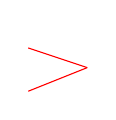
\begin{tikzpicture}
    \draw (-1,1) -- (-1,1);
    \begin{scope}[color=red]
      \draw (-1,0.75) -- (-0.25,0.5);
      \draw (-1,0.2) -- (-0.25,0.5);
    \end{scope}
  \end{tikzpicture}}

\begin{table}
  \begin{whole}
  \begin{tabular}{rrrclrrrr}

    &
    &
    &
    \multicolumn{2}{c}{$Mdn_{\sum{E}}$} \\

    &
    \multicolumn{1}{c}{$N$} &
    \multicolumn{1}{c}{$Mdn$} &
    \multicolumn{2}{c}{$- Mdn_{\sum{C}}$} &
    \multicolumn{1}{c}{$Rng$} &
    \multicolumn{1}{c}{$U$} &
    \multicolumn{1}{c}{$Z$} &
    \multicolumn{1}{c}{$p$ (1-tailed)} \\

    \cmidrule(lr){2-9}

    $E$ &
    12 &
    5 &
    \multirow{2}{*}{\twoguides} &
    \multirow{2}{*}{1} &
    4 &
    \multirow{2}{*}{45} &
    \multirow{2}{*}{-1.353} &
    \multirow{2}{*}{0.089}\\

    $C$ &
    11 &
    4 &
    &
    &
    3 \\

  \end{tabular}
  \caption[Up-to-date on Favorites' Activities, Between Groups]{%
    Up-to-date on favorites' activities. Comparison between
    experiment and control group for the posttest.
  }
  \label{table:uptodate.favorite.activities.between}
  \end{whole}
\end{table}

The results show that the median degree of acceptance to the statement
is higher for experiment respondents having used an activity stream than
control respondents with a placebo. This difference is however
not statistically significant.

We also tested if there was a change in acceptance within the respondent
groups from before they were given a treatment or placebo and after.
The results can be seen in
\tableref{uptodate.favorite.activities.within}.

\newcommand{\fourguides}{%
  \begin{tikzpicture}
    \draw (-1,1) -- (-1,1);
    \begin{scope}[color=red]
      \draw (-1,0.5) -- (-0.25,0);
      \draw (-1,-0.5) -- (-0.25,-0);
    \end{scope}
    \draw (-1,-1) -- (-1,-1);
  \end{tikzpicture}}

\begin{table}
  \begin{whole}
  \begin{tabular}{rrrrccclrrrr}

    &
    &
    &
    &
    \multicolumn{2}{c}{Post} &
    \multicolumn{2}{c}{$Mdn_{\sum{E}}$} \\

    &
    &
    \multicolumn{1}{c}{$N$} &
    \multicolumn{1}{c}{$Mdn$} &
    \multicolumn{2}{c}{$-$ Pre} &
    \multicolumn{2}{c}{$- Mdn_{\sum{C}}$} &
    \multicolumn{1}{c}{$Rng$} &
    \multicolumn{1}{c}{$T$} &
    \multicolumn{1}{c}{$Z$} &
    \multicolumn{1}{c}{$p$ (1-tailed)} \\

    \cmidrule(lr){3-12}

    \multirow{2}{*}{$E$} &
    Pre &
    14 &
    3 &
    \multirow{2}{*}{\twoguides} &
    \multirow{2}{*}{2} &
    \multirow{4}{*}{\fourguides} &
    \multirow{4}{*}{1} &
    4 &
    \multirow{2}{*}{10} &
    \multirow{2}{*}{-1.513} &
    \multirow{2}{*}{0.086}\\

    &
    Post &
    12 &
    5 &
    &
    &
    &
    &
    4 \\

    \multirow{2}{*}{$C$} &
    Pre &
    11 &
    3 &
    \multirow{2}{*}{\twoguides} &
    \multirow{2}{*}{1} &
    &
    &
    3 &
    \multirow{2}{*}{16} &
    \multirow{2}{*}{-0.787} &
    \multirow{2}{*}{0.258}\\

    &
    Post &
    11 &
    4 &
    &
    &
    &
    &
    3 \\

  \end{tabular}
  \caption[Up-to-date on Favorites' Activities, Within Groups]{%
    Up-to-date on favorites' activities.  Comparison between
    pretest and posttest within the experiment and control group.
  }
  \label{table:uptodate.favorite.activities.within}
  \end{whole}
\end{table}

The data shows that the median acceptance rate have rosen from the pretest to
the posttest for both experiment and control respondents. The acceptance of
the statemnent about how easy it is to keep up-to-date on favorites'
activities have rosen more for the respondents having used an activity stream
than those with a placebo. Neither of these increases of median values
are statistically significant.

\parabreak

While we observed increases in how easy respondents felt they could keep
up-to-date with favorites' activities when an activity stream was used,
none of this data was statistically significant. Due to lack of evidence we
can not reject $H_0$.

%%
%% Move this hypothesis (non) rejection part together with next results
%%

Based on the statements:
\begin{items}
  \item It's easy to keep up-to-date on whether my favorites publishes
    new songs on \urort{}.
  \item It's easy to keep up-to-date on whether my favorites publishes
    new blog posts on \urort{}.
  \item It's easy to keep up-to-date on whether my favorites are
    performing at concerts.
  \item It's easy to keep up-to-date on the reactions other users at
    \urort{} have towards my favorite artists' songs.
\end{items}

we graded respondents answers as follows:

\begin{items}
  \item Fully disagree: 1
  \item Somewhat disagree: 2
  \item Neither agree nor disagree: 3
  \item Somewhat agree: 4
  \item Fully agree: 5
\end{items}

The $H_0$ stated that we would not see any positive change in how easy
respondents felt it was to keep up-to-date on favorites' specific activities
after introducing an activity steam. Our $H_A$ said that we
would indeed observe a change in how respondents rated this task.

First we compared how easy responents felt it was to keep up-to-date on
favorites' specific activities after they are given a treatment
or a placebo.
See
\tableref{uptodate.favorite.specific.activities.between} for the results.

\begin{table}
  \begin{whole}
  \begin{tabular}{rrrclrrrrl}

    &
    &
    &
    \multicolumn{2}{c}{$Mdn_{\sum{E}}$} \\

    &
    \multicolumn{1}{c}{$N$} &
    \multicolumn{1}{c}{$Mdn$} &
    \multicolumn{2}{c}{$- Mdn_{\sum{C}}$} &
    \multicolumn{1}{c}{$Rng$} &
    \multicolumn{1}{c}{$U$} &
    \multicolumn{1}{c}{$Z$} &
    \multicolumn{1}{c}{$p$ (1-tailed)} \\

    \cmidrule(lr){2-9}

    $E$ &
    12 &
    5 &
    \multirow{2}{*}{\twoguides} &
    \multirow{2}{*}{1,0} &
    4 &
    \multirow{2}{*}{59} &
    \multirow{2}{*}{-0.479} &
    \multirow{2}{*}{0.340} &
    \multirow{2}{*}{Song}\\

    $C$ &
    11 &
    4 &
    &
    &
    2 \\

    \cmidrule(lr){2-9}

    $E$ &
    12 &
    4.5 &
    \multirow{2}{*}{\twoguides} &
    \multirow{2}{*}{1.5} &
    4 &
    \multirow{2}{*}{59} &
    \multirow{2}{*}{-0.460} &
    \multirow{2}{*}{0.289} &
    \multirow{2}{*}{Blog}\\

    $C$ &
    11 &
    3 &
    &
    &
    2 \\

    \cmidrule(lr){2-9}

    $E$ &
    12 &
    3.5 &
    \multirow{2}{*}{\twoguides} &
    \multirow{2}{*}{-0.5} &
    4 &
    \multirow{2}{*}{66} &
    \multirow{2}{*}{0.000} &
    \multirow{2}{*}{0.517} &
    \multirow{2}{*}{Concert}\\

    $C$ &
    11 &
    4 &
    &
    &
    3 \\

    \cmidrule(lr){2-9}

    $E$ &
    12 &
    3.5 &
    \multirow{2}{*}{\twoguides} &
    \multirow{2}{*}{0.5} &
    4 &
    \multirow{2}{*}{60} &
    \multirow{2}{*}{-0.385} &
    \multirow{2}{*}{0.372} &
    \multirow{2}{*}{Review}\\

    $C$ &
    11 &
    3 &
    &
    &
    3 \\

  \end{tabular}
  \caption[Up-to-date on Favorites' Specific Activities, Between Groups]{%
    Up-to-date on favorites' specific activities. Comparison between
    experiment and control group for the posttest.
  }
  \label{table:uptodate.favorite.specific.activities.between}
  \end{whole}
\end{table}

The reported median degree of how easy it is to keep up-to-date
on new songs, blogs posts, and reviews is higher for those
which used an activity stream than those without. Respondents using
and activity stream reported a lower median value of how easy it was
to keep up-to-date on concerts compared to those without such treatment.
Neither the increases and decreases in the median degree from the
control group to the experiment group were stastically significant.

As for general activities we also tested whether respondents perception
of how easy it was to keep up-to-date on specific activities from
favorites had changed from before a treatment or placebo was given to after.
See 
\tableref{uptodate.favorite.specific.activities.within} for the results of the
in group comparisons.

\begin{table}
  \begin{whole}
  \begin{tabular}{rrrrccclrrrrl}

    &
    &
    &
    &
    \multicolumn{2}{c}{Post} &
    \multicolumn{2}{c}{$Mdn_{\sum{E}}$} \\

    &
    &
    \multicolumn{1}{c}{$N$} &
    \multicolumn{1}{c}{$Mdn$} &
    \multicolumn{2}{c}{$-$ Pre} &
    \multicolumn{2}{c}{$- Mdn_{\sum{C}}$} &
    \multicolumn{1}{c}{$Rng$} &
    \multicolumn{1}{c}{$T$} &
    \multicolumn{1}{c}{$Z$} &
    \multicolumn{1}{c}{$p$ (1-tailed)} \\

    \cmidrule(lr){3-12}

      \multirow{2}{*}{$E$} &
        Pre &
        14 &
        4 &
        \multirow{2}{*}{\twoguides} &
        \multirow{2}{*}{1} &
        \multirow{4}{*}{\fourguides} &
        \multirow{4}{*}{0} &
        4 &
        \multirow{2}{*}{8.0} &
        \multirow{2}{*}{-1.780} &
        \multirow{2}{*}{0.049} &
        \multirow{4}{*}{Song} \\

        &
        Post &
        12 &
        5 &
        &
        &
        &
        &
        4 \\

      \multirow{2}{*}{$C$} &
        Pre &
        11 &
        3 &
        \multirow{2}{*}{\twoguides} &
        \multirow{2}{*}{1} &
        &
        &
        3 &
        \multirow{2}{*}{4.0} &
        \multirow{2}{*}{-1.709} &
        \multirow{2}{*}{0.055} &
        \\

        &
        Post &
        11 &
        4 &
        &
        &
        &
        &
        2 \\

    \cmidrule(lr){2-12}

      \multirow{2}{*}{$E$} &
        Pre &
        14 &
        3 &
        \multirow{2}{*}{\twoguides} &
        \multirow{2}{*}{1.5} &
        \multirow{4}{*}{\fourguides} &
        \multirow{4}{*}{1.5} &
        3 &
        \multirow{2}{*}{9.5} &
        \multirow{2}{*}{-1.872} &
        \multirow{2}{*}{0.039} &
        \multirow{4}{*}{Blog} \\

        &
        Post &
        12 &
        4.5 &
        &
        &
        &
        &
        4 \\

      \multirow{2}{*}{$C$} &
        Pre &
        11 &
        3 &
        \multirow{2}{*}{\twoguides} &
        \multirow{2}{*}{0} &
        &
        &
        3 &
        \multirow{2}{*}{13.0} &
        \multirow{2}{*}{-1.150} &
        \multirow{2}{*}{0.166} &
        \\

        &
        Post &
        11 &
        3 &
        &
        &
        &
        &
        2 \\

    \cmidrule(lr){2-12}

      \multirow{2}{*}{$E$} &
        Pre &
        14 &
        3 &
        \multirow{2}{*}{\twoguides} &
        \multirow{2}{*}{0.5} &
        \multirow{4}{*}{\fourguides} &
        \multirow{4}{*}{-0.5} &
        3 &
        \multirow{2}{*}{7.5} &
        \multirow{2}{*}{-1.127} &
        \multirow{2}{*}{0.188} &
        \multirow{4}{*}{Concert} \\

        &
        Post &
        12 &
        3.5 &
        &
        &
        &
        &
        4 \\

      \multirow{2}{*}{$C$} &
        Pre &
        11 &
        3 &
        \multirow{2}{*}{\twoguides} &
        \multirow{2}{*}{1} &
        &
        &
        3 &
        \multirow{2}{*}{5.5} &
        \multirow{2}{*}{-1.063} &
        \multirow{2}{*}{0.203} &
        \\

        &
        Post &
        11 &
        4 &
        &
        &
        &
        &
        3 \\

    \cmidrule(lr){2-12}

      \multirow{2}{*}{$E$} &
        Pre &
        13 &
        3 &
        \multirow{2}{*}{\twoguides} &
        \multirow{2}{*}{0.5} &
        \multirow{4}{*}{\fourguides} &
        \multirow{4}{*}{1.5} &
        4 &
        \multirow{2}{*}{4.5} &
        \multirow{2}{*}{-1.298} &
        \multirow{2}{*}{0.125} &
        \multirow{4}{*}{Review} \\

        &
        Post &
        12 &
        3.5 &
        &
        &
        &
        &
        4 \\

      \multirow{2}{*}{$C$} &
        Pre &
        11 &
        4 &
        \multirow{2}{*}{\twoguides} &
        \multirow{2}{*}{-1} &
        &
        &
        3 &
        \multirow{2}{*}{9.5} &
        \multirow{2}{*}{-0.780} &
        \multirow{2}{*}{0.281} &
        \\

        &
        Post &
        11 &
        3 &
        &
        &
        &
        &
        3 \\

  \end{tabular}
  \caption[Up-to-date on Favorites' Specific Activities, Within Groups]{%
    Up-to-date on favorites's specific activities. Comparison between
    pretest and posttest within the experiment and control group.
  }
  \label{table:uptodate.favorite.specific.activities.within}
  \end{whole}
\end{table}

The within group data shows that experiment respondents and control
respondents find it easier to keep up-to-date on rencent songs
and concert performances after the treatment or placebo was given.
The increases are of the same order for both those which used an
activity stream and those without. Neither of the two groups increases
for concerts is statistically significant.
The experiment groups' increase is significant for songs while the control
groups' increase for songs is insignificant.
Note that the difference between $p$ values for the two groups related to
songs are marginal.

Respondents having used an activity stream saw an increase in median
response from \q{neither agree or disagree} to \q{fully agree} regarding
how easy it was to keep up-to-date on blog posts of favorites.
This difference is statistically significant.
The control group saw no such increase after they were given a placebo.

On the topic of how easy respondents could keep up-to-date on
reviews of favorites' songs the experiment group saw no change
after treatment while the control group saw a decrease after having used
a placebo. This decrease is not statistically significant.

\parabreak

None of the differences we found with regards to specific activities between
the experiment and control group for the posttest was significant.
We can't reject $H_0$ for any of the specific activities based on this
evidence. Well look at how $H_0$ stands based on the difference within groups
from before treatment and placebo were given to after for each specific
activity:

\begin{items}
  \iterm{Song:} We did find significant evidence
    of a an increase in ease of keeping up-to-date on songs for respondents
    which used an activity stream while those without had insignificant
    increases. The difference of significance were quite small so $H_0$
    stands unrejected for songs.
  \iterm{Blog:} The respondents which had used an activity list saw a
    significant increase in their median ranks of how easy it was
    to keep up-to-date on blogs. The respondents having used our placebo
    saw no such increase. Based on this evidence we reject $H_0$ in favor
    of $H_A$ for keeping up-to-date on blog posts.
  \iterm{Concert:} Both experiment and control groups saw
    statistically insignificant increases in their median degree of how easy
    the task was for concerts. $H_0$ therefore stands unrejected for concerts.
  \iterm{Review:} For reviews we noticed no significant increases or decreases
    of the median degree of how easy it was to keep up-to-date. 
    $H_0$ therefore stands unrejected for reviews.
\end{items}

%%
%% perceived usefulness results
%%

%%
%% perceived ease-of-use results
%%

%%
%% rejection or non-rejection of the H0 here after listing all results
%%

\subsubsection{%
  Does social navigation trough activity streams lead users to more often keep
  up-to-date on favorites' activities on \urort{}?
}

Based on the question
\q{How often do you update yourself on what your favorites on \urort{}
   are doing?}
we graded respondents answers as follows: 

\begin{items}
  \item Daily: 5
  \item Several times a week: 4
  \item Weekly: 3
  \item Monthly: 2
  \item Seldom/never: 1
\end{items}

Our $H_0$ stated that we would not see any increase in how frequent
experiment respondents kept up-to-date on favorites' activities after giving
them an activity feed. The alternative $H_A$ contradicted this and said
an activity feed would increase the frequency experiment respondents were
keeping up-to-date.

First we compared how frequent respondents having used an activity feed kept
up-to-date with those which hadn't used an activity feed. The results are
displayed in \tableref{uptodate.favorite.activities.frequency.between}.

\begin{table}
  \begin{whole}
  \begin{tabular}{rrrclrrrr}

    &
    &
    &
    \multicolumn{2}{c}{$Mdn_{\sum{E}}$} \\

    &
    \multicolumn{1}{c}{$N$} &
    \multicolumn{1}{c}{$Mdn$} &
    \multicolumn{2}{c}{$- Mdn_{\sum{C}}$} &
    \multicolumn{1}{c}{$Rng$} &
    \multicolumn{1}{c}{$U$} &
    \multicolumn{1}{c}{$Z$} &
    \multicolumn{1}{c}{$p$ (1-tailed)} \\

    \cmidrule(lr){2-9}

    $E$ &
    13 &
    2 &
    \multirow{2}{*}{\twoguides} &
    \multirow{2}{*}{-1} &
    2 &
    \multirow{2}{*}{24.5} &
    \multirow{2}{*}{-2.955} &
    \multirow{2}{*}{0.002}\\

    $C$ &
    11 &
    3 &
    &
    &
    2 \\

  \end{tabular}
  \caption[Up-to-date on Favorites' Activities Frequency,
           Between Groups]{%
    Frequency of keeping up-to-date on favorites' activities. Comparison
    between experiment and control group for the posttest.
  }
  \label{table:uptodate.favorite.activities.frequency.between}
  \end{whole}
\end{table}

As can be seen from the data respondents which had used an activity feed
reported lower median frequencies of use than those which had used a placebo.
This difference is higly significant.

As for our previous two research questions and hypotheses we've also checked
if there were changes in the frequency of keeping up-to-date within the
experiment and control groups from before they were given a treatment or
placebo to after.
The results can be seen in
\tableref{uptodate.favorite.activities.frequency.within}.

\begin{table}
  \begin{whole}
  \begin{tabular}{rrrrccclrrrr}

    &
    &
    &
    &
    \multicolumn{2}{c}{Post} &
    \multicolumn{2}{c}{$Mdn_{\sum{E}}$} \\

    &
    &
    \multicolumn{1}{c}{$N$} &
    \multicolumn{1}{c}{$Mdn$} &
    \multicolumn{2}{c}{$-$ Pre} &
    \multicolumn{2}{c}{$- Mdn_{\sum{C}}$} &
    \multicolumn{1}{c}{$Rng$} &
    \multicolumn{1}{c}{$T$} &
    \multicolumn{1}{c}{$Z$} &
    \multicolumn{1}{c}{$p$ (1-tailed)} \\

    \cmidrule(lr){3-12}

    \multirow{2}{*}{$E$} &
    Pre &
    13 &
    1 &
    \multirow{2}{*}{\twoguides} &
    \multirow{2}{*}{1} &
    \multirow{4}{*}{\fourguides} &
    \multirow{4}{*}{1} &
    2 &
    \multirow{2}{*}{10} &
    \multirow{2}{*}{-1.941} &
    \multirow{2}{*}{0.046}\\

    &
    Post &
    13 &
    2 &
    &
    &
    &
    &
    2 \\

    \multirow{2}{*}{$C$} &
    Pre &
    11 &
    3 &
    \multirow{2}{*}{\twoguides} &
    \multirow{2}{*}{0} &
    &
    &
    2 &
    \multirow{2}{*}{8} &
    \multirow{2}{*}{-1.134} &
    \multirow{2}{*}{0.227}\\

    &
    Post &
    11 &
    3 &
    &
    &
    &
    &
    2 \\

  \end{tabular}
  \caption[Up-to-date on Favorites' Activities Frequency, Within Groups]{%
    Frequency of keeping up-to-date on favorites' activities. Comparison
    between pretest and posttest within the experiment and control group.
  }
  \label{table:uptodate.favorite.activities.frequency.within}
  \end{whole}
\end{table}

The results show a different picture than the between group posttest results.
Here we see that the frequency of keeping up-to-date have increased over time
for those respondents which used an activity feed. Those respondents with a
placebo show a stagnation in the frequency of keeping up-to-date.
The increase for experiment respondents is statistically significant.

\parabreak

Based on our comparison of frequency of keeping up-to-date between experiment
and control groups for the posttest alone, our $H_0$ seems to still hold true.
But if one take into the account the differences in frequency of keeping
up-to-date between the two groups from the pretest the data indicates
an increase in frequency of keeping up-to-date for only those respondents
having used an activity feed. We can therefore reject our $H_0$ in favor
of the $H_A$ for frequency of keeping up-to-date.


\subsection{Favorite usage}

\subsubsection{%
  Does social navigation trough activity streams lead users to make
  more artists on \urort{} their favorites?
}

%%
%% results from favorite numbers
%%
